\documentclass[captions=tableheading]{scrartcl}

\usepackage{amsmath}
\usepackage{amssymb}
\usepackage[utf8]{inputenc}
\usepackage[T1]{fontenc}
\usepackage{lmodern}
\usepackage{ngerman}
\usepackage{geometry}
\usepackage{graphicx}
\usepackage{wrapfig}
\usepackage{caption}
\usepackage{wasysym}
\usepackage[separate-uncertainty=true]{siunitx}
\usepackage{picinpar}
\usepackage{tikz}
\usepackage{float}
\usepackage{booktabs}
\usepackage{enumitem} 

\renewcommand{\figurename}{Abb.}
\usepackage[
	colorlinks=true,
	urlcolor=blue,
	linkcolor=black
]{hyperref}


%Hier Titel und so
\newcommand{\versuchnummer}{V60} 
\newcommand{\versuchname}{Der Diodenlaser} 
\newcommand{\versuchdatum}{23.01.2017} 

\let\oldsection\section
\renewcommand\section{\clearpage\oldsection}

\title{Versuch \versuchnummer\\ \versuchname}
\subtitle{Physikalisches Fortgeschrittenenpraktikum}
\author{Robert Rauter und Björn Lindhauer}
\date{\versuchdatum} 
\begin{document}
\begin{titlepage}
{\large \versuchdatum}
\vspace{7cm}
\begin{center}
\textbf{\huge Versuch \versuchnummer}\\\vspace{0.5cm}
\textbf{\huge \versuchname}\\
\vspace{0.2cm}
\textbf{Physikalisches Fortgeschrittenenpraktikum}\\
\vspace{9cm}

{\Large Robert Rauter \ \ \hspace{1.5cm} und \hspace{1.5cm} Björn Lindhauer}\\
{ \url{robert.rauter@tu-dortmund.de} \ \ \hspace{2cm} \url{bjoern.lindhauer@tu-dortmund.de}}
\end{center}
\end{titlepage}

\section{Grundlagen}
Der Diodenlaser ist ein Halbleiterbauteil, welches einen Laserstrahl erzeugen kann. Im Folgenden soll die Funktionsweise des Diodenlasers kurz skizziert werden und die Möglichkeiten der Abstimmung des Lasers aufgezeigt werden.
\subsection{Struktur}
Der Diodenlaser liegt in Form eines Chips vor, welcher auf einen Kühlkörper befestigt wird und durch kleine Kabel verbunden wird. Der Aufbau des Chips ist in Abbildung $\ref{fig:aufbau_diodenlaser}$ dargestellt. 
\begin{center}
	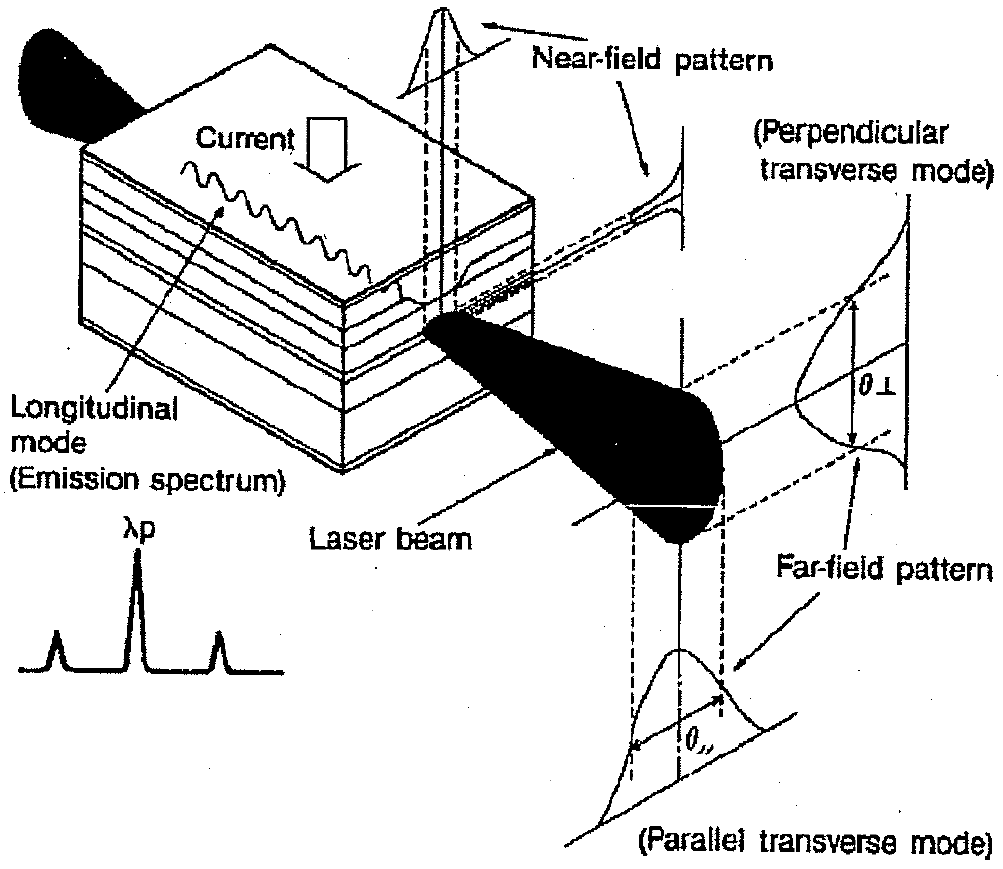
\includegraphics[width=10cm]{images/aufbau_diodenlaser.png}
	\captionof{figure}{Schematischer Aufbau des Chips \ref{q:anleitung}}
	\label{fig:aufbau_diodenlaser}
\end{center}
Wird nun eine Spannung am Chip angelegt, so entstehen Elektronen-Loch-Paare.
Diese rekombinieren in der aktiven Schicht und emittieren dabei Licht.
Das Licht wird in kleinen Kanal in der Grö"senordnung $2\times 10 \times 400\si{\micro\meter}$  eingeschlossen. 
Die Facetten am Ende des Kanals bilden teilweise reflektierende Flächen, sodass ein Resonator entsteht.

Der Chip besteht aus n- und p-notierten Schichten, deshalb Elektronen rekombinieren an den Verbindungsflächen von den p und n Schichten. 
Somit ist in erster Näherung die Wellenlänge des emittierten Lichts gleich der Bandlücke.

Der Resonator in der Diode kann so konstruiert werden, dass nur longitudinale Moden im Resonator ausgebildet werden. 
Diese Dioden haben typischerweise eine Bandbreite von $\Delta \nu \sim \SI{50}{\mega\hertz}$.
\newpage
Ein Diodenlaser ist abhängig von der angelegten Spannung. Ist die Spannung zu klein, so ist der Verlust grö"ser als der Verstärkungsgrad (gain) des Resonators und es wird keine Besetzungsinversion erreicht. Das emittierte Licht entsteht nur durch die spontane Emission und ist somit breitbandig.
Überschreitet die Spannung einen Schwellwert, so wird ein kohärenter Strahl aus dem Laser emittiert, da die induzierte Emission überliegt. 
Die Intensität des Stahls wächst linear mit der Spannung und dabei erreicht der Diodenlaser eine Effektivität von $\sim 50\%$.

Der Strahl ist dabei aufgrund des rechteckigen Kanals, wie in Abbildung \ref{fig:aufbau_diodenlaser} dargestellt, elliptisch und divergiert. 
Deswegen wird eine Sammellinse in den Strahl gesetzt.

Die große Frequenzbreite $\Delta \nu$ des Strahles und optische Rückkopplungen sorgen für Instabilitäten in der Frequenz. Dies lässt sich mit Hilfe eines Beugungsgitters, welches einen kleinen Teil ($\sim 15\%$) des Strahles rückkoppeln. Es entsteht somit ein weiterer externer Resonator, der die Bandweite auf $\Delta\nu\sim\SI{1}{\mega\hertz}$ senkt. Der gesamte Aufbau ist in Abbildung \ref{fig:aufbau_linsen} dargestellt. 
\begin{center}
	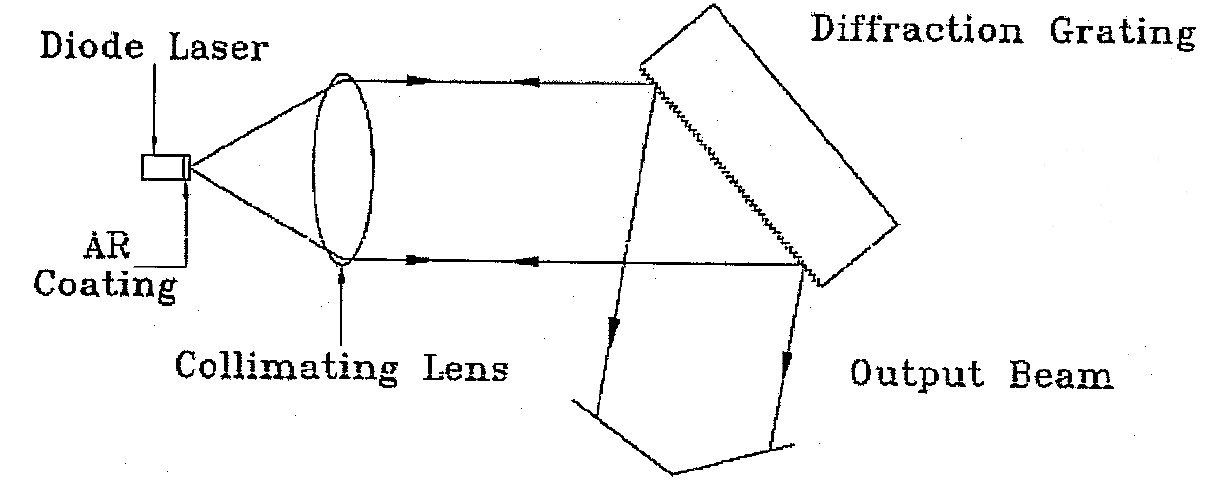
\includegraphics[width=12cm]{images/aufbau_linse.png}
	\captionof{figure}{Schematischer Aufbau des Laser-Systems \ref{q:anleitung}}
	\label{fig:aufbau_linsen}
\end{center}

\subsection{Abstimmen des Lasers} 
Es gibt verschiedene Parameter, mit denen der Laser abgestimmt werden kann. Eine Übersicht ist in Abbildung \ref{fig:gainwavelength} gegeben. 
Dabei tendiert der Laser in der Mode mit den höchsten optischen Gesamtverstärkungsgrad zu arbeiten.
Denn die Anzahl der Elektron-Loch-Paare für das Lasern in anderen Moden ist durch die stimulierte Emission stark beschränkt und der Laser kann somit nur in einer Mode arbeiten. 
Im Folgenden werden die einzelnen Beiträge separat diskutiert.

\begin{center}
	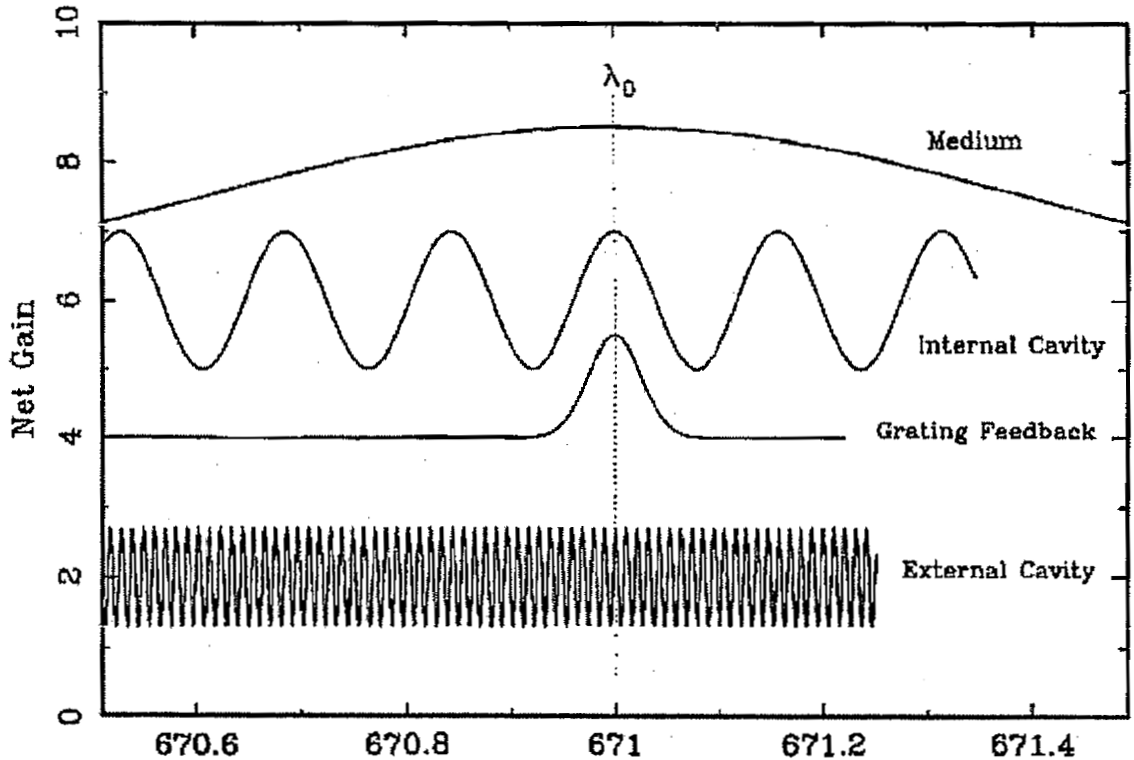
\includegraphics[width=10.5cm]{images/gainwavelength.png}
	\captionof{figure}{Beiträge zum Gesamtverstärkungsgrad \ref{q:anleitung}}
	\label{fig:gainwavelength}
\end{center}

\subsubsection{Medium}
Wie bereits zu Begin erwähnt, hängt die Frequenz des erzeugten Stahls von der Bandlücke ab. 
Im Frequenzraum ist der Verstärkungsgrad des Mediums ein stark abgeflachter Peak. 
Die Position des Peaks hängt stark von der Temperatur ab, denn die Resonatorlänge unterliegt thermischen Schwankungen. 
Da in diesen Versuch die Rubidium Spektrallinie aufgenommen werden soll, muss die Temperatur so gewählt werden, dass der Laser nahe $\SI{780}{\nano\meter}$  arbeitet.
\begin{center}
	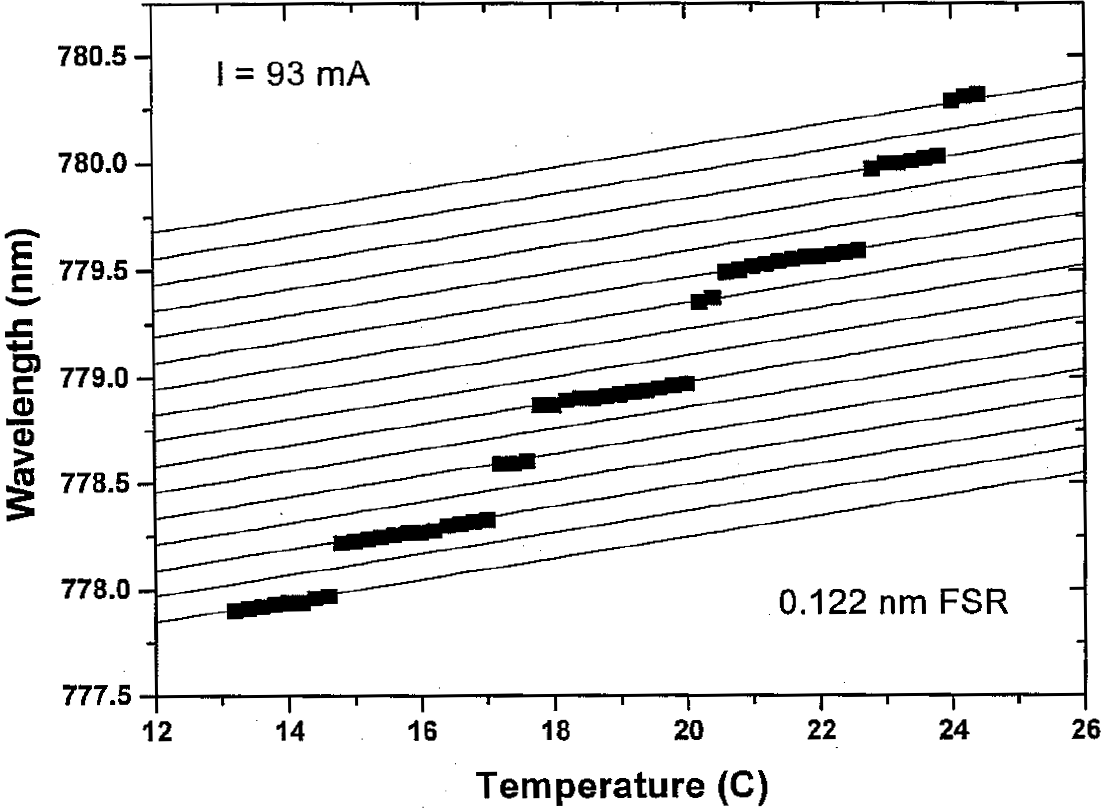
\includegraphics[width=10.5cm]{images/temperatur.png}
	\captionof{figure}{Temperaturabhängigkeit der Wellenlänge \ref{q:anleitung}}
	\label{fig:temperatur}
\end{center}
Die Temperaturabhängigkeit der Wellenlänge ist in Abbildung \ref{fig:temperatur} dargestellt. 
Die Sprünge der Kurve werden als \textit{mode hops} bezeichnet. 
Die Steigung dieser Kurve liegt bei etwa $\SI{0.23}{\nano\meter\per\kelvin}$ und somit ist diese Kurve so flach, dass die Temperatur nicht für die genaue Abstimmung relevant ist. 

\subsubsection{Optische Resonatoren}
Die Verbindungsflächen der Schichten in der Diode bilden bekanntermaßen einen optischen Resonator und hat folglich auch eine Normalmodenstruktur.
Deshalb ist der daraus resultierende Gesamtverstärkungsgrad periodisch in der Frequenz. 
Die Periode ist durch
\begin{align*}
\Delta \nu_{\text{FSR}}=\frac{c}{2Ln}
\end{align*}
gegeben mit der Lichtgeschwindigkeit $c$, den Brechungsindex $n$ und der Resonatorlänge $L$. 
Die Periode wird auch \textit{free spectral range} genannt.
In diesem Experiment liegt diese bei $\Delta \nu_{\text{FSR}} \approx \SI{60}{\giga\hertz}$. 
Die Verstärkung ist temperatur- und spannungsabhängig, wie in Abbildung \ref{fig:spannung} zu sehen. 

Dies liegt daran, dass bei steigender Spannung die Temperatur im Chip erhöht wird. Außerdem ändert die Spannung die Konzentration der Elektronen, die zur Bildung der Elektron-Loch-Paare benötigt werden.   
\begin{center}
	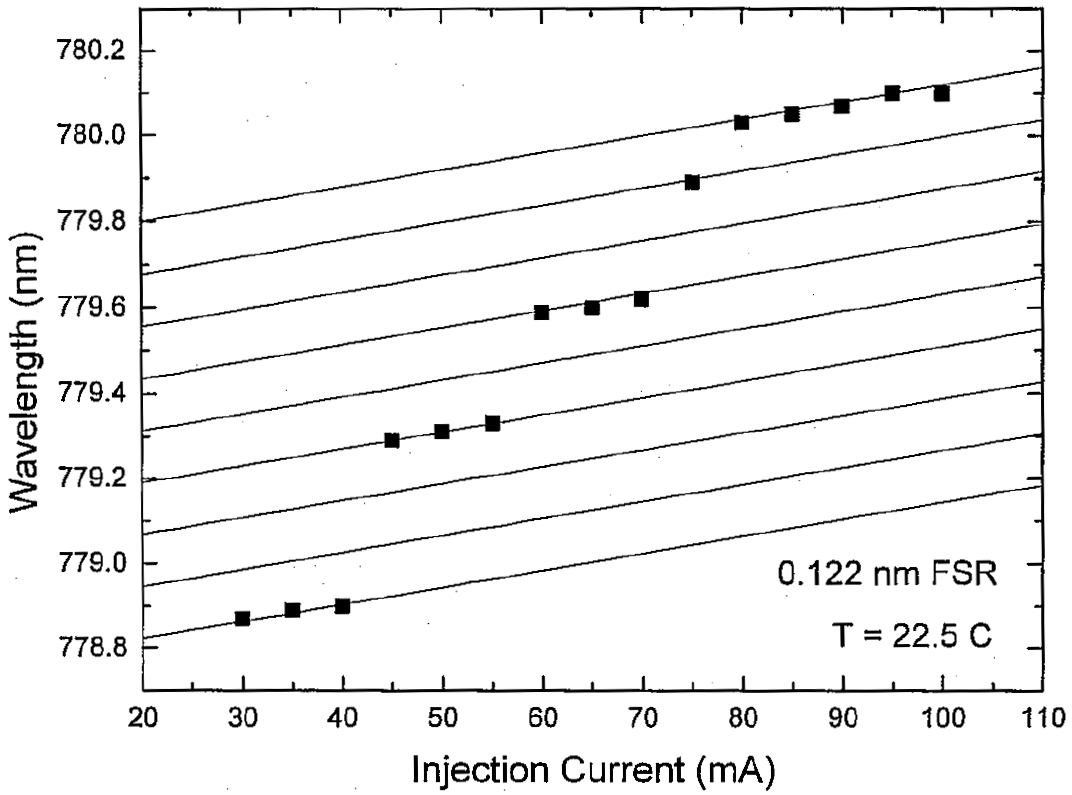
\includegraphics[width=10.5cm]{images/spannung.png}
	\captionof{figure}{Spannungsabhängigkeit der Wellenlänge \ref{q:anleitung}}
	\label{fig:spannung}
\end{center}
Der externe Resonator funktioniert wie der interne Resonator mit dem Unterschied, dass die Länge $L\approx\SI{15}{\milli\meter}$ größer ist und somit $\Delta \nu_{\text{FSR}} \approx \SI{10}{\giga\hertz}$. 

Um die Wellenlänge genau einzustellen, ist das Beugungsgitter nötig.
\newpage
\subsubsection{Beugungsgitter}
 Der verwendete Aufbau wird auch als Littrow-Konfiguration bezeichnet. 
 Für einen festen Winkel zur Horizontalen wird nur Licht mit bestimmter Wellenlänge, die in einen kleinen Bereich liegt, reflexiert. 
 Die Wellenlänge ist durch 
\begin{align*}
\lambda=2d\sin\Theta 
\end{align*}  
 gegeben, wobei $d$ die Gitterkonstante und $\Theta$ der Winkel des Gitters ist.
 Bei einen Idealen Gitter ist die Spektralbreite durch
 \begin{align*}
 \frac{\nu}{\Delta \nu}=N
\end{align*}  
gegeben. Dabei ist $N$ die Anzahl der Gitterlinien, die den Strahl reflexieren.
\subsubsection{Zusammenwirken der Beiträge}

Die Abbildung \ref{fig:gainsimple} gibt ein Überblick über die verschiedenen Beiträge. 
Dabei wurde der Verstärkungsgrad des Medium weggelassen. 
Außerdem wurde der Verstärkungsgrad der Reflexion am Gitter und des externen Resonators in einer gemeinsamen Funktion dargestellt. 
Der Laser würde in diesen Fall in der Frequenz arbeiten, bei der beide Verstärkungsgrade ihr Maximum besitzen.
\begin{center}
	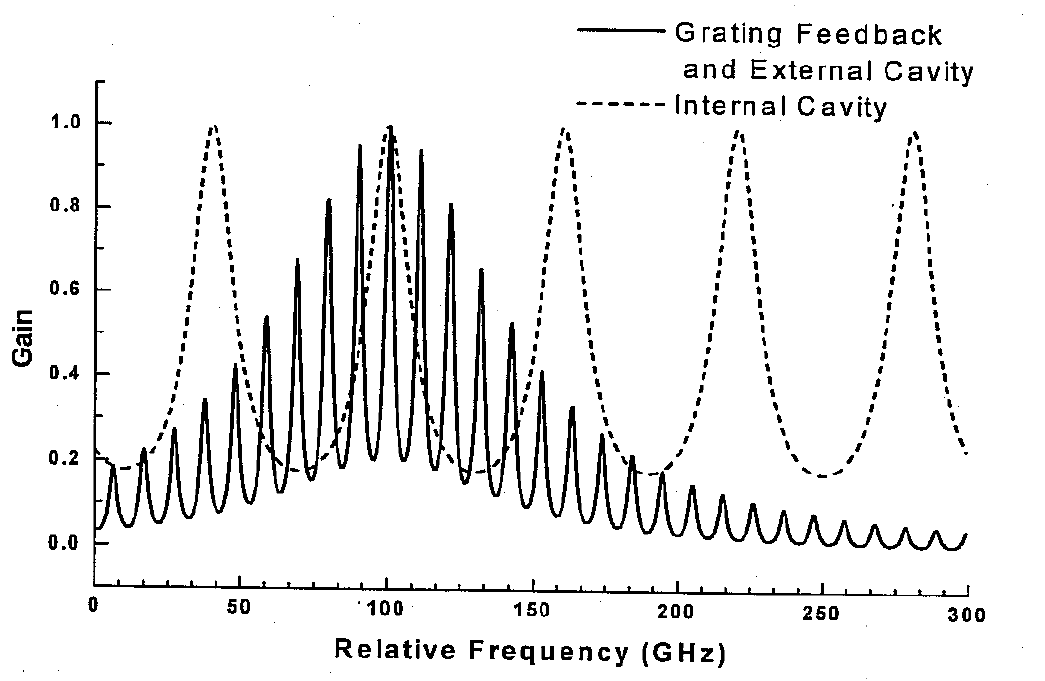
\includegraphics[width=10.5cm]{images/gainsimple.png}
	\captionof{figure}{Verstärkungsgrad des internen Resonators, der Reflexion am Gitter und des externen Resonators in Abhängigkeit der Frequenz \ref{q:anleitung}}
	\label{fig:gainsimple}
\end{center}
Die Abbildung \ref{fig:gainmulti} zeigt die Moden in Abhängigkeit des Rotationswinkels $\Theta$ des Gitters. 
Es sind die beiden internen Moden $Int0$ und $Int1$, sowie mehrere externe Moden $e0$, $e1$ usw. eingetragen. 
\newpage
Beim Graphen a ist das Maximum des Verstärkungsgrad der beiden Kurven an der gleichen Frequenz. Der Laser ist in der Mode $e0$. 
Wird der Winkel des Gitters verkleinert, so wandert die Mode $e0$ zu höheren Frequenzen. 
Wie in Graph b dargestellt, existiert ein Winkel, an den $Int0$ zwischen $e-1$ und $e0$ liegt.
Es wird die Mode $e0$ bei kleineren Winkeln immer instabiler gegenüber Mode $e-1$, bis es zum Phasensprung kommt.

Die Graphen c und d zeigen eine andere Art von Phasensprung. Dabei wird nicht die benachbarte externe Mode bevorzugt, sondern eine andere Mode, die durch die interne Mode $Int1$ bevorzugt wird. 

Es können folglich viele verschiedene Moden durch den Winkel des Gitters eingestellt werden. 
\begin{center}
	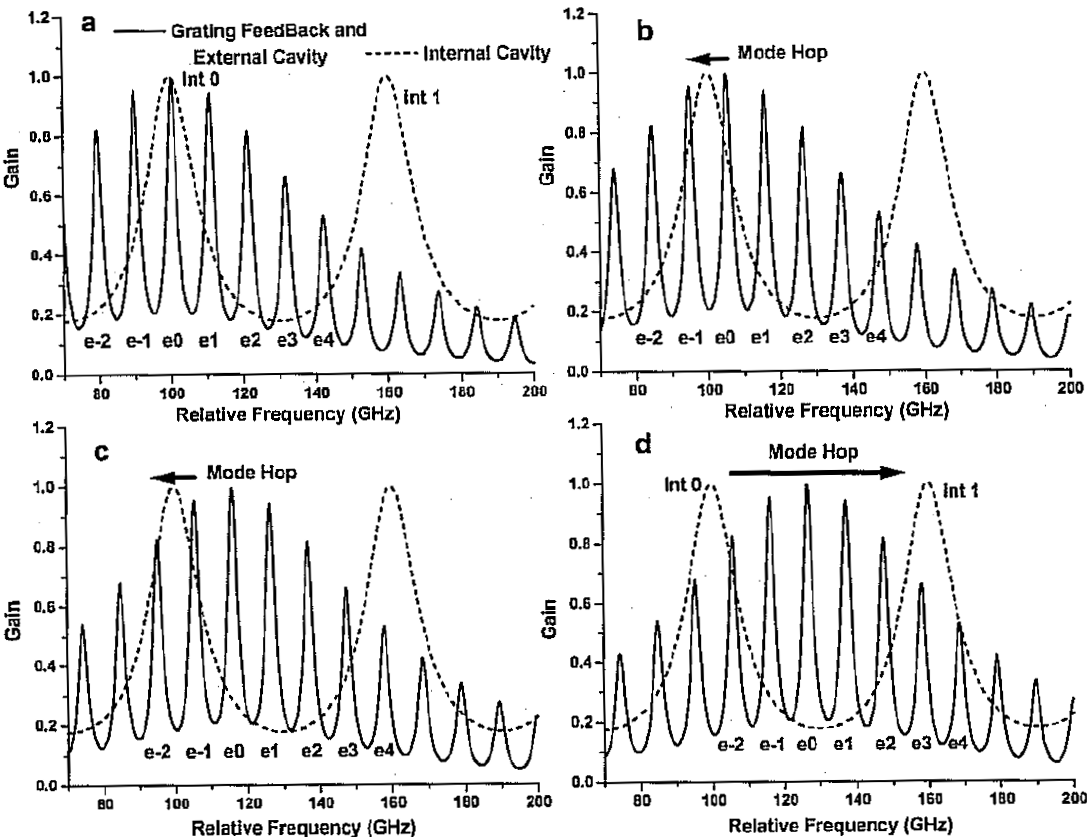
\includegraphics[width=15cm]{images/gainmulti.png}
	\captionof{figure}{Verstärkungsgrad des internen Resonators, der Reflexion am Gitter und des externen Resonators in Abhängigkeit der Frequenz für verschiedene Winkel $\Theta$ des Gitters \ref{q:anleitung}}
	\label{fig:gainmulti}
\end{center}
 
\newpage
\section{Aufbau}

\subsection{Justierung des Strahlengangs}
Zur Justierung des Strahlengangs wird eine Laserdetektionskarte in den Strahlengang gehalten und eine Videokamera auf die Photozelle gerichtet. \\
Zur Justierung des Strahlenganges sind zwei Drehschrauben am Diodenlaser vorhanden, jeweils für die horizontale und die vertikale Justierung.
 
\subsection{Beobachtung der Rubidium-Resonanz}
In Abbildung \ref{fig:setup} ist das Setup zur Detektion der Rubidium-Fluoreszenz dargestellt.
\begin{center}
	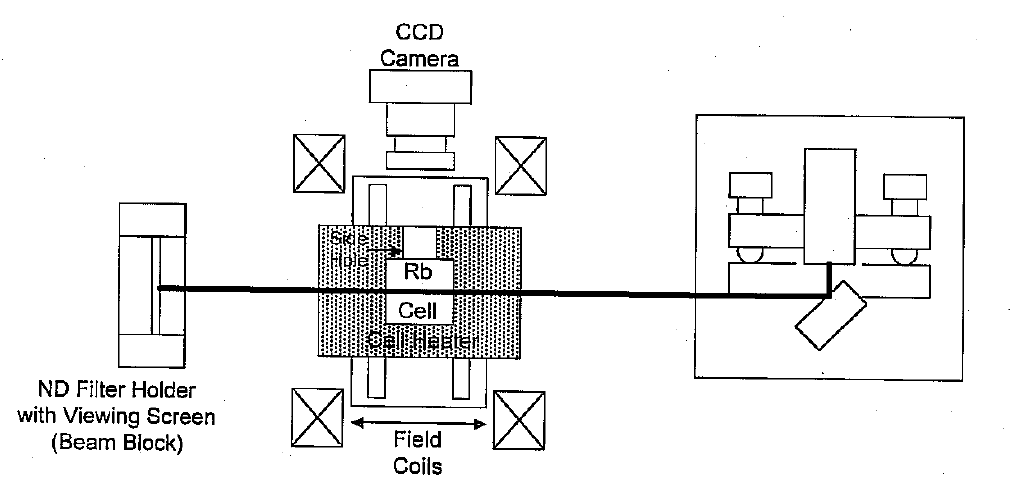
\includegraphics[width=10cm]{images/setup.png}
	\captionof{figure}{Setup zur Detektion von Rubidium-Fluoreszenz \ref{q:anleitung}}
	\label{fig:setup}
\end{center}
Zur Detektion der Fluoreszenz wird der horizontale Winkel des Gitters schrittweise angepasst. Die Feinabstimmung wird durch eine Anpassung der Piezospannung erreicht. Im Falle einer Resonanz kann diese mit der Kamera und des Oszilloskop detektiert werden. \\

\section{Durchführung}

\subsection{Justierung des Strahlengangs}
Mithilfe einer Kamera kann das Verhalten des Strahls bei Variation der Stromstärke beobachtet werden. Unterhalb des Grenzwertes der Stromstärke verhält sich der Diodenlaser wie eine LED, d.h. es kommt zu spontaner Emission. Ein Bild es entstehenden Signals ist in Abbildung \ref{fig:led} zu sehen.
\begin{center}
	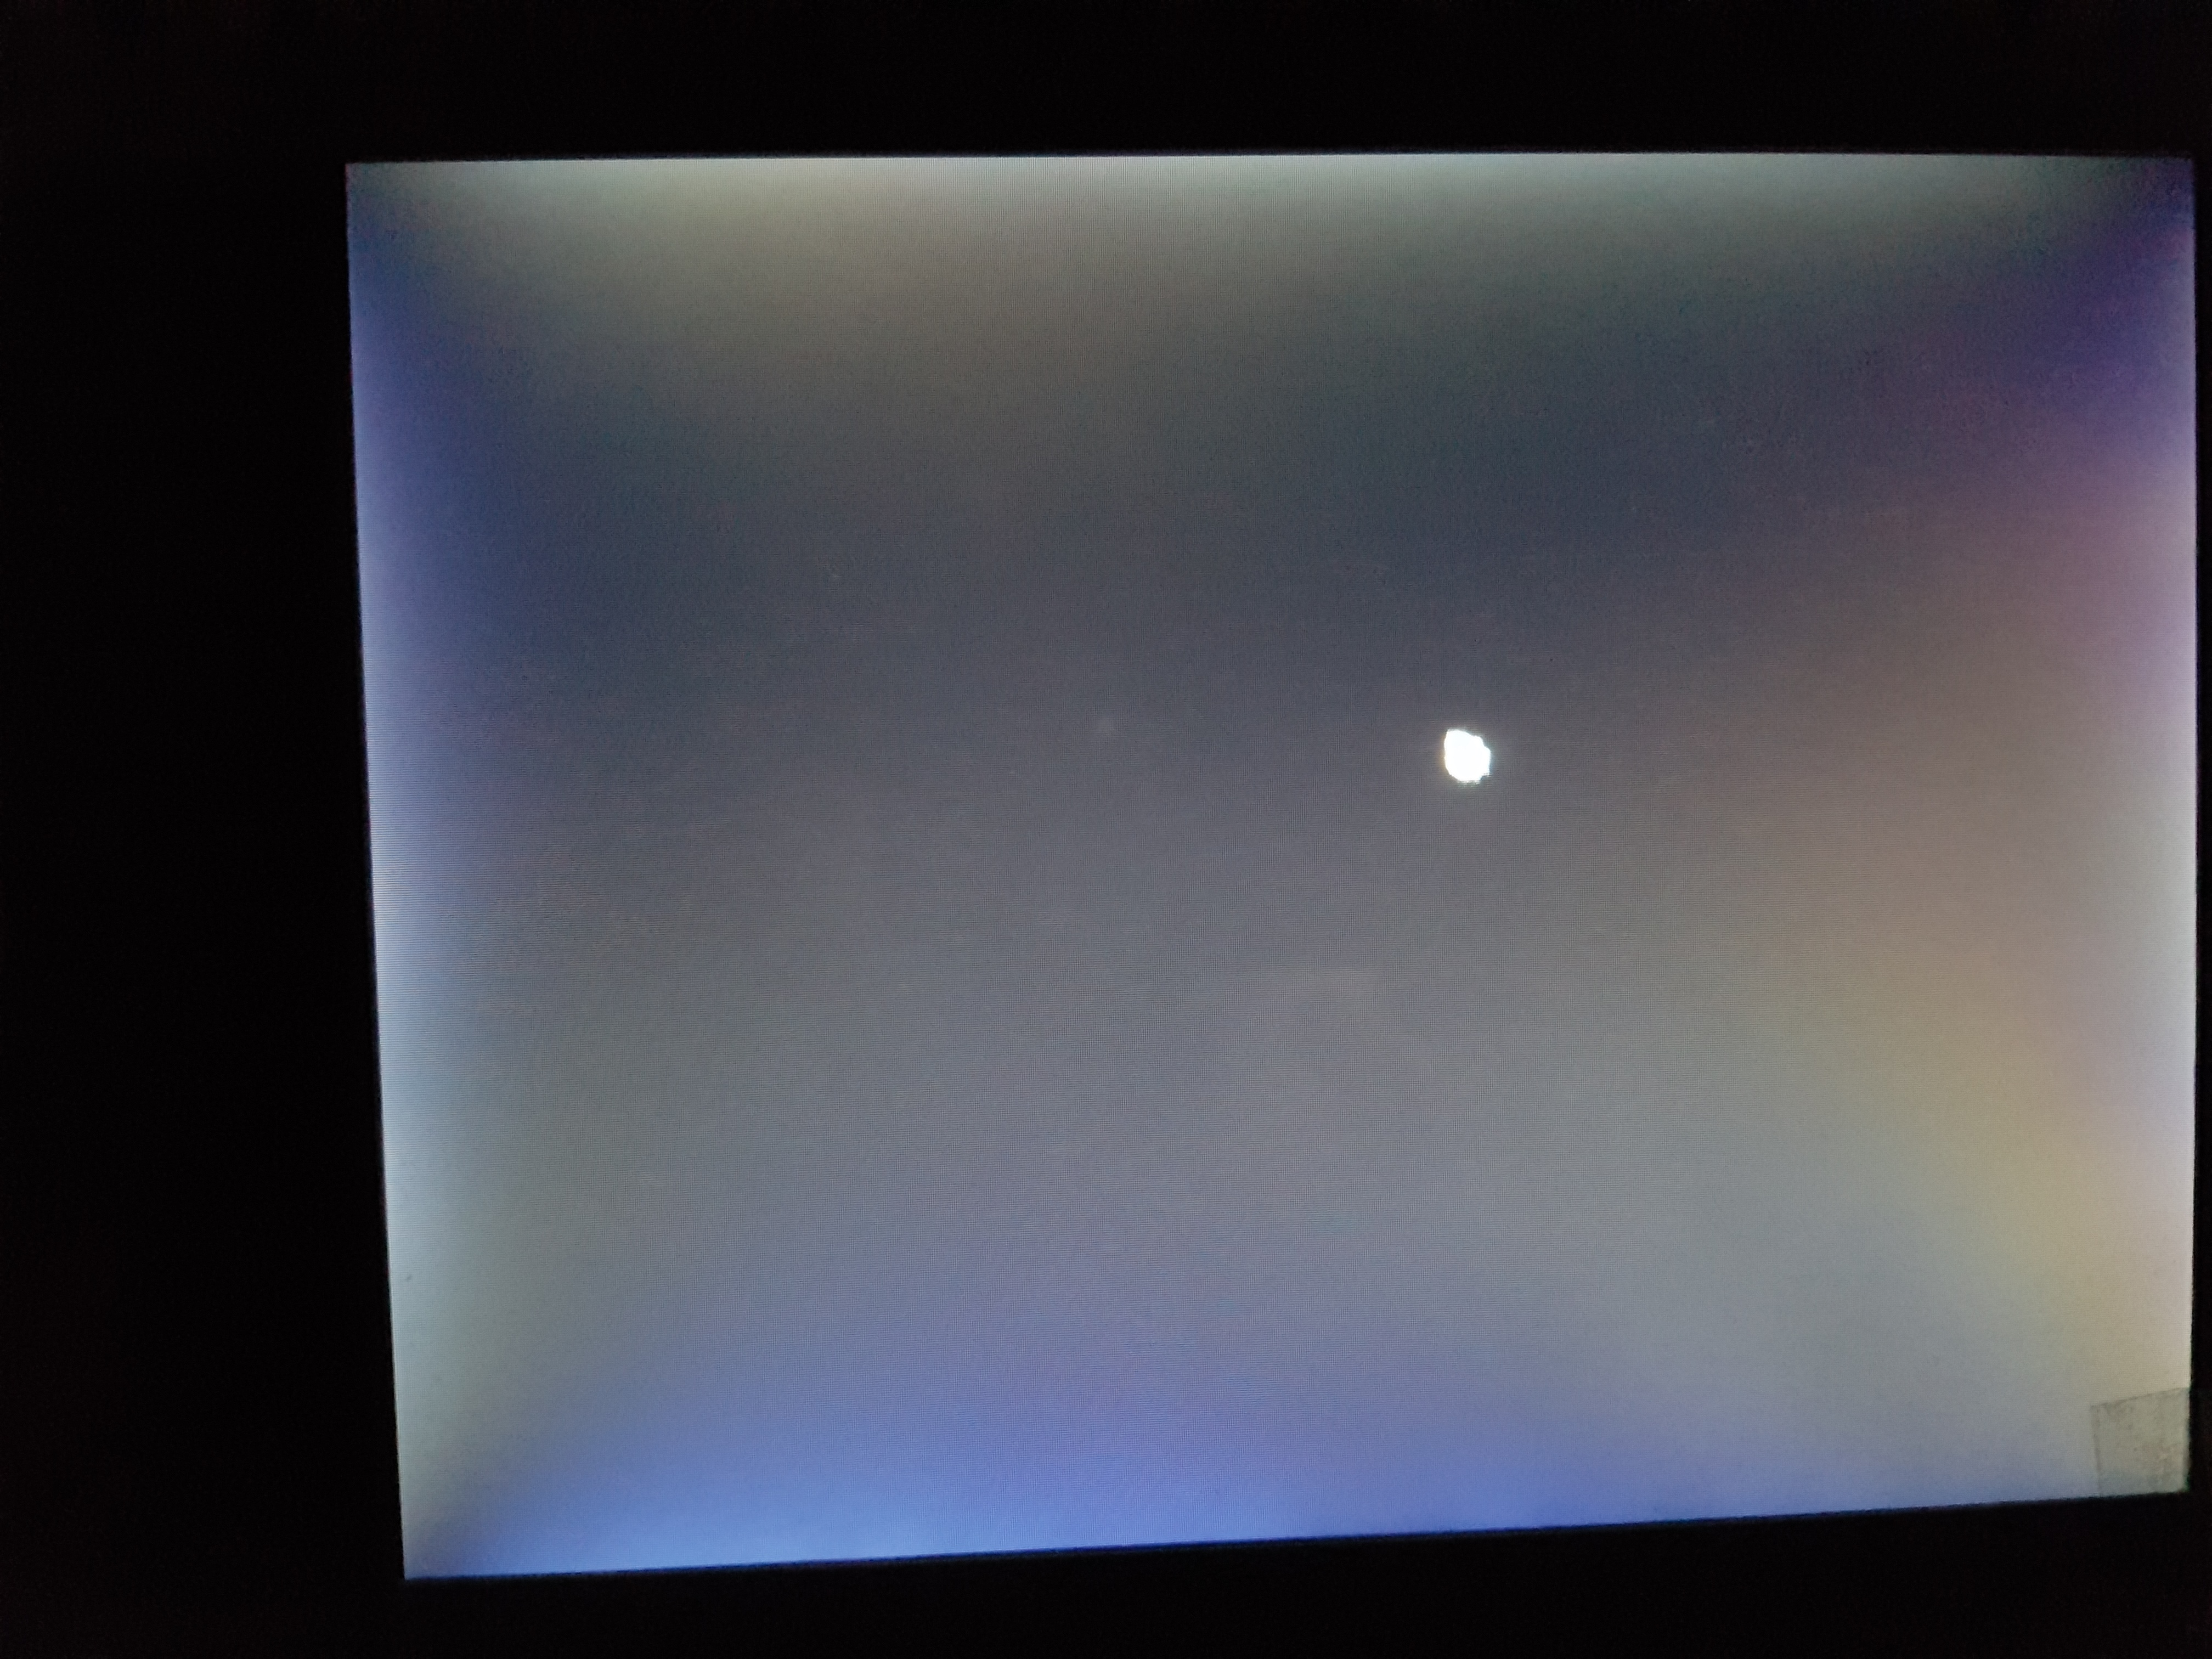
\includegraphics[width=10cm]{images/led_spot.jpg}
	\captionof{figure}{Beobachtetes Ausgangssignal des Diodenlasers unterhalb der Grenzstromstärke}
	\label{fig:led}
\end{center}
Wird der Grenzwert der Stromstärke überschritten, tritt eine deutliche Erhöhung der Strahlintensität auf, wie es in Abbildung \ref{fig:over_threshold} zu sehen ist. 
\newpage
\begin{center}
	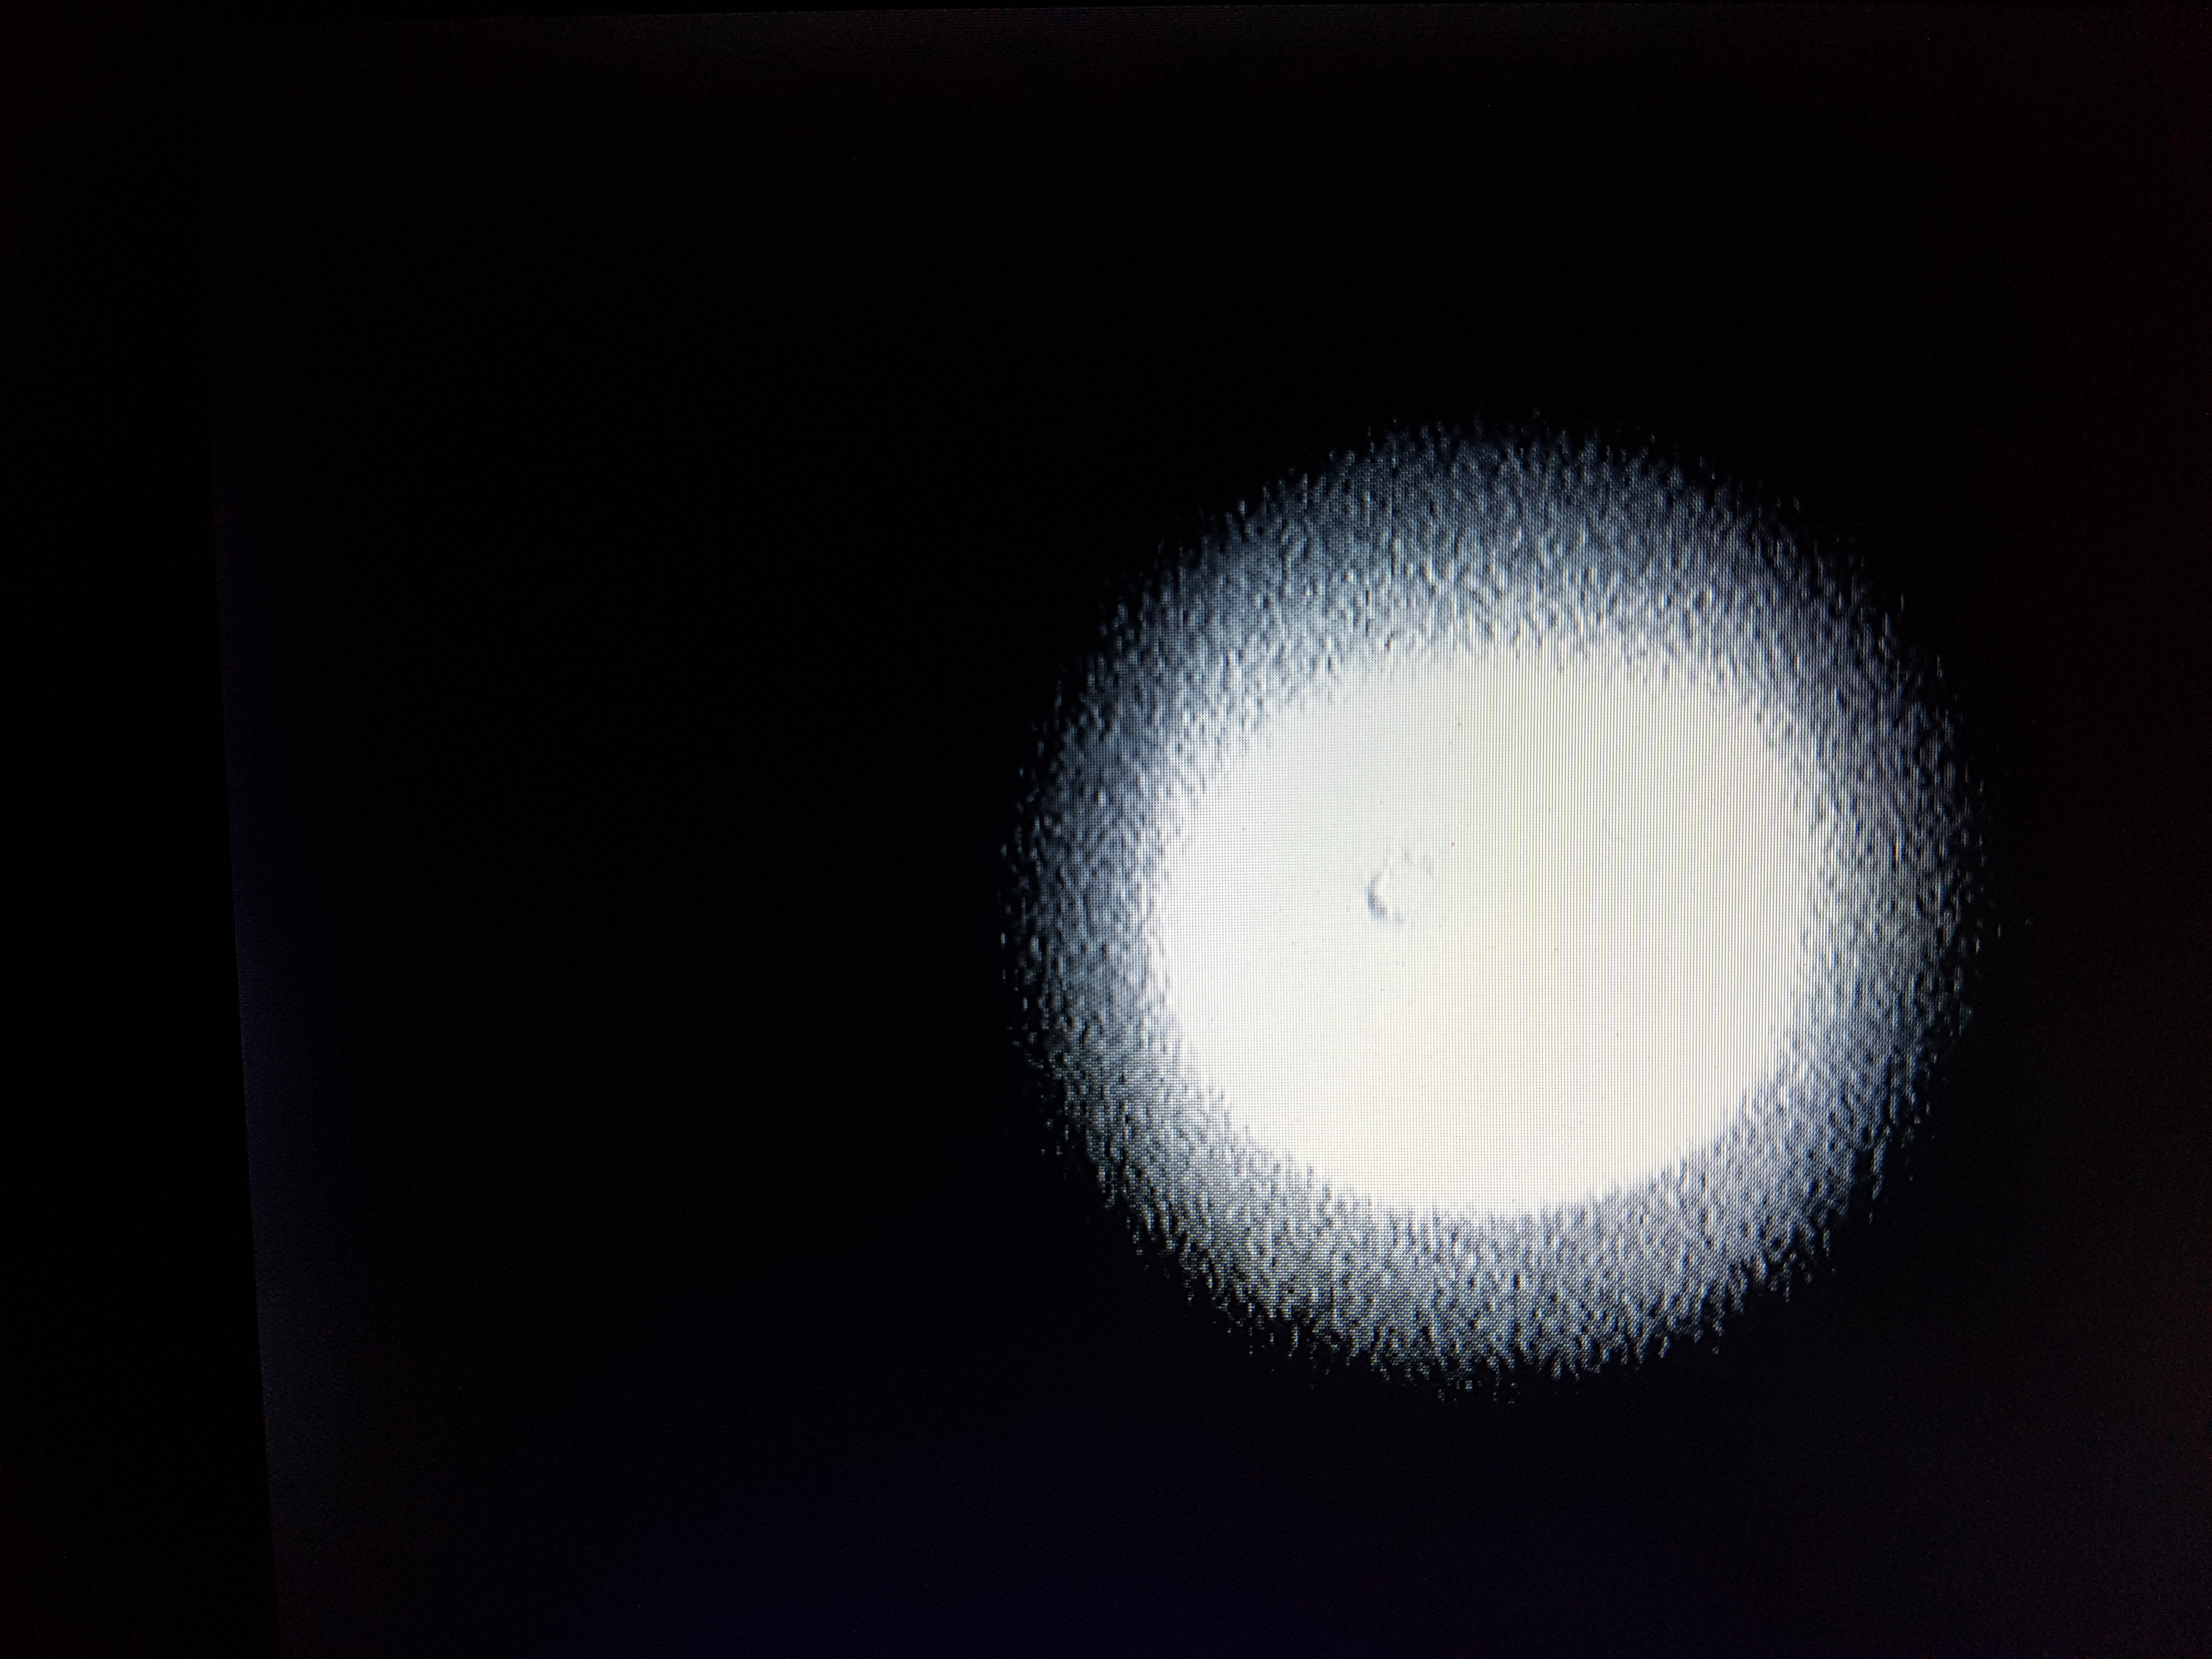
\includegraphics[width=10cm]{images/over_threshold.jpg}
	\captionof{figure}{Beobachtetes Ausgangssignal des Diodenlaser oberhalb der Grenzstromstärke}
	\label{fig:over_threshold}
\end{center}

\subsection{Beobachtung der Rubidium-Resonanz}
Mithilfe des im Kapitel 3 beschriebenen Aufbaus kann die Rubidium-Resonanz mittels einer Kamera beobachtet werden. Dies ist in Abbildung \ref{fig:resonanzbild} abgebildet.
\begin{center}
	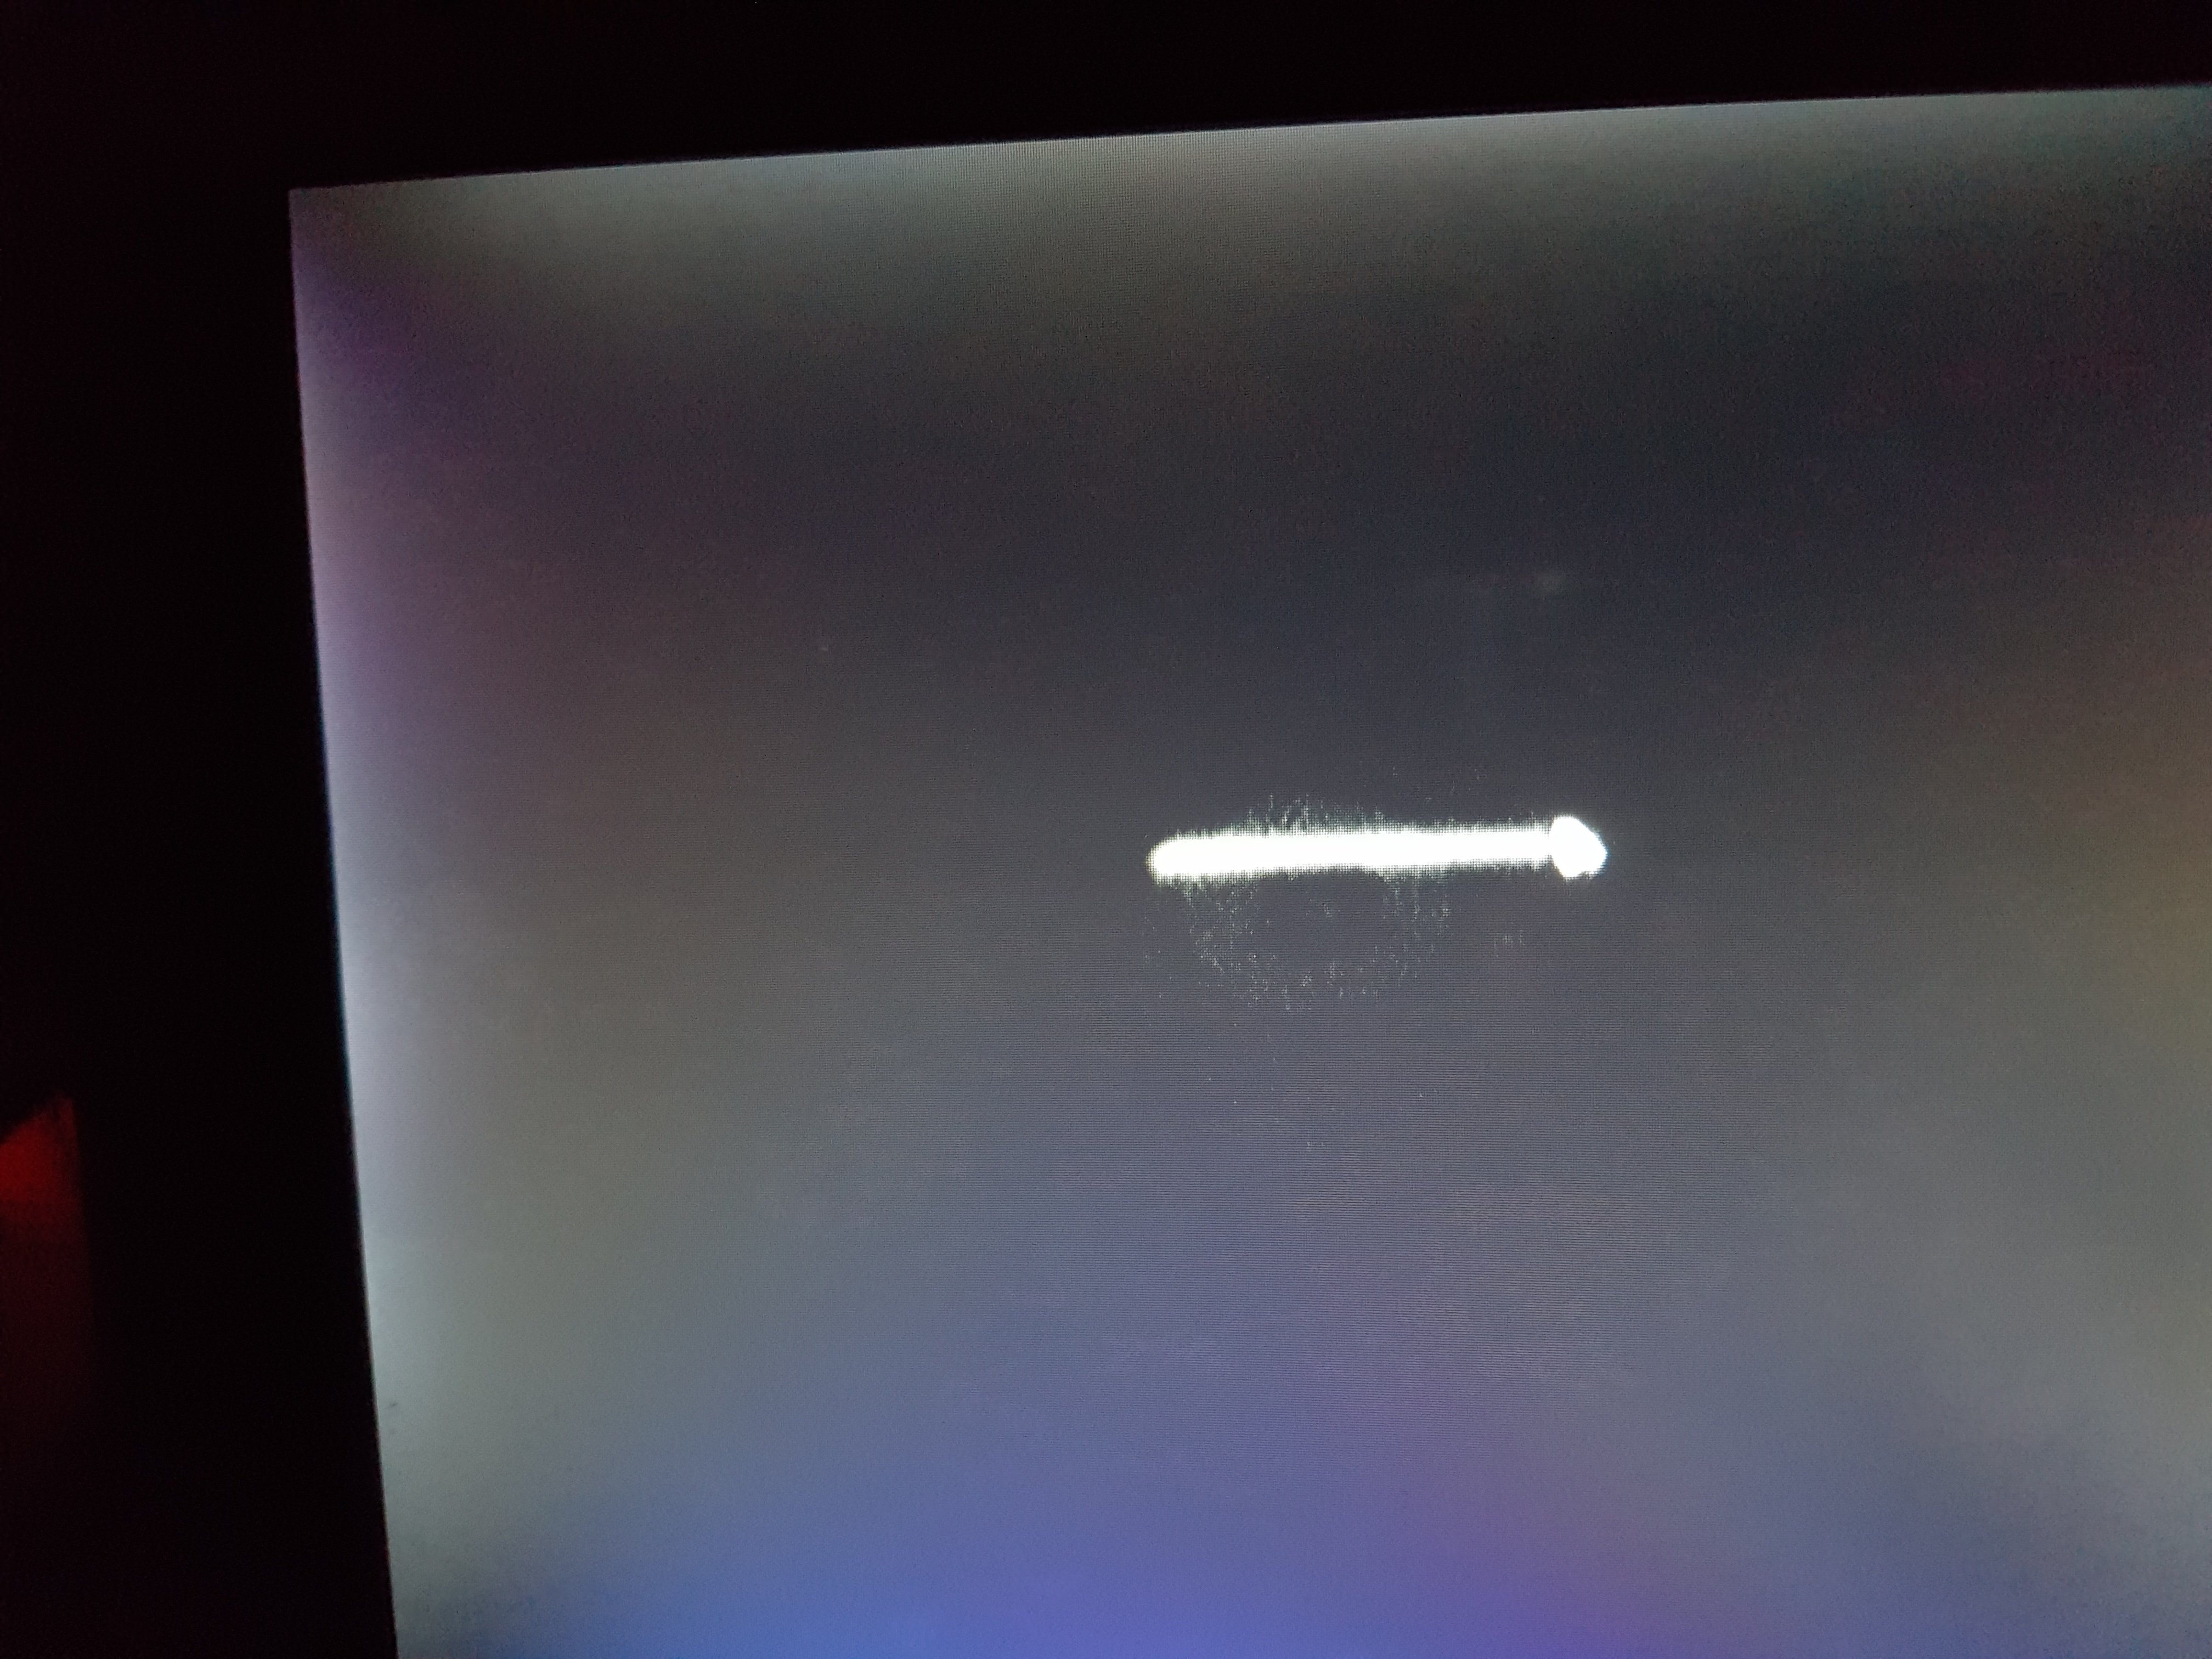
\includegraphics[width=10cm]{images/resonanz_bild.jpg}
	\captionof{figure}{Mit Kamera detektiertes Resonanzsignal}
	\label{fig:resonanzbild}
\end{center}
Um die Intensität zu verringern, wird ein Dämpfungsglied in den Strahlengang gestellt. Das Signal der Photodiode wird mithilfe eines Photodetektors detektiert und auf einem Oszilloskop dargestellt. 
\begin{center}
	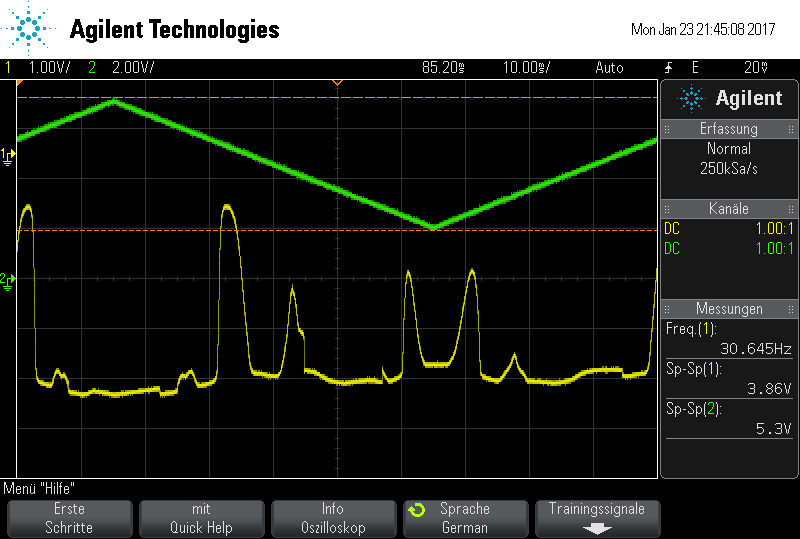
\includegraphics[width=10cm]{images/scope_22.png}
	\captionof{figure}{Resonanzspektrum von Rubidium}
	\label{fig:resonanz}
\end{center}
Das grüne Dreiecksignal ist die Spannung, die am Piezoelement anliegt, welches die Orientierung des Gitters bestimmt und somit die Frequenzen durchscannt. Das gelbe Signal zeigt die Absorptionspeaks der Photozelle, die durch den Rubidium-Dampf erzeugt werden.

\subsection{Bereinigung des Resonanzsignals}
Zur Bereinigung des Resonanzsignals von z.B. der Spannungsmodulation des Piezokristalles, wird mithilfe der Differenzspannungsmethode der Hintergrund des Signals entfernt. In Abbildung \ref{fig:resonanzlinien} ist dabei das Absorptionssignal ohne Hintergrundbereinigung dargestelt, in Abbildung \ref{fig:resonanzlinien_mh} das finale Signal ohne Hintergrund.
\begin{center}
	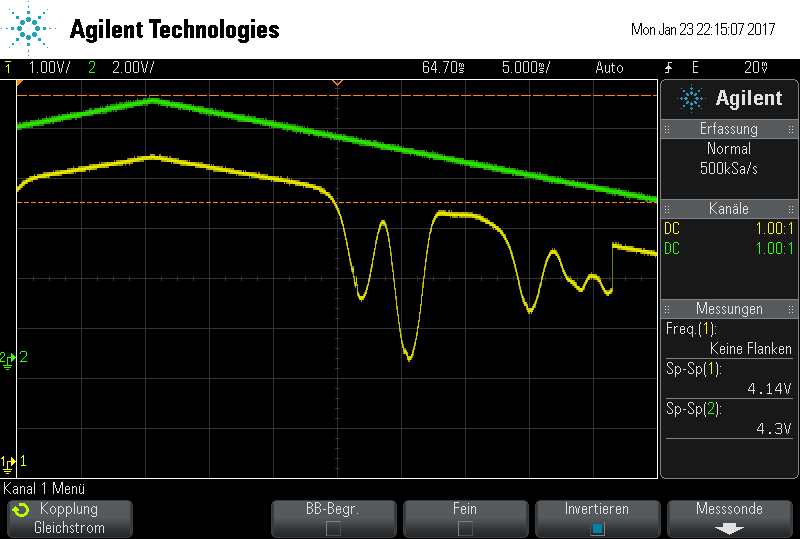
\includegraphics[width=10cm]{images/resonanz.png}
	\captionof{figure}{Resonanzlinien der Rubidium-Probe, mit Hintergrund-Intensität}
	\label{fig:resonanzlinien}
\end{center}

\begin{center}
	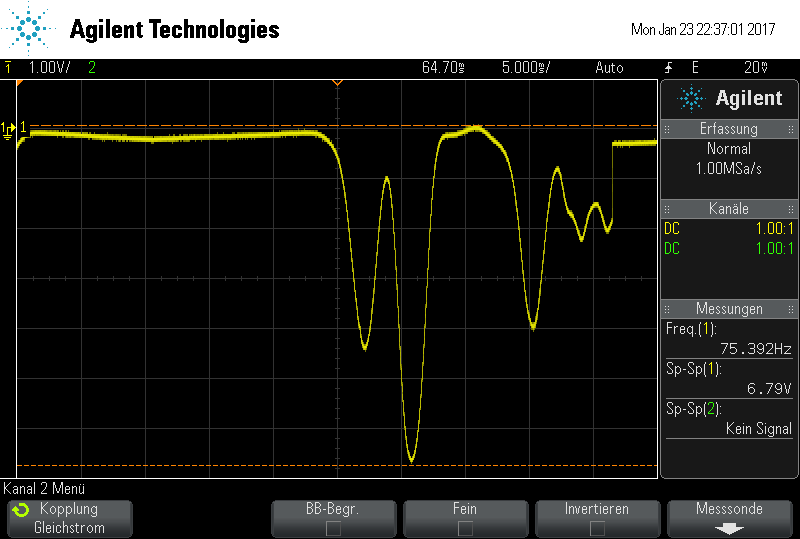
\includegraphics[width=10cm]{images/resonanz_bereinigt.png}
	\captionof{figure}{Um Hintergrund bereinigte Resonanzlinien der Rubidium-Probe}
	\label{fig:resonanzlinien_mh}
	\end{center}

\section{Diskussion}
Nach der Justierung des Strahlenganges konnte eine hohe Intensität des Strahls erreicht werden. Desweiteren wurde eine starke Resonanzintensität des Rubidiumdampfes erreicht. \\
Die Resonanzlinien des Rubidiumdampfes ($^{85}$Rb und $^{87}$Rb) konnten klar abgebildet werden, wobei die Resonanzspitzen gau"sverbreitert waren. Zusätzlich dazu konnten zwei "'extra features"' im Spektrum zu entdecken gewesen. \\


\section{Quellen}
%\renewcommand{\labelenumi}{\value{enumi}}
\begin{enumerate}[label={[\arabic*]}]
\item \label{q:anleitung} \textbf{Physikalisches Praktikum}, TU Dortmund: \\
\textit{Versuchsanleitung zu Versuch 60: Der Diodenlaser} \\
\url{http://129.217.
224.2/HOMEPAGE/PHYSIKER/MASTER/SKRIPT/V60.pdf} (letzte Version vom 24.01.2017, 16:00)
\end{enumerate}


\end{document}